\begin{textblock}{8.}(0., -4.)
    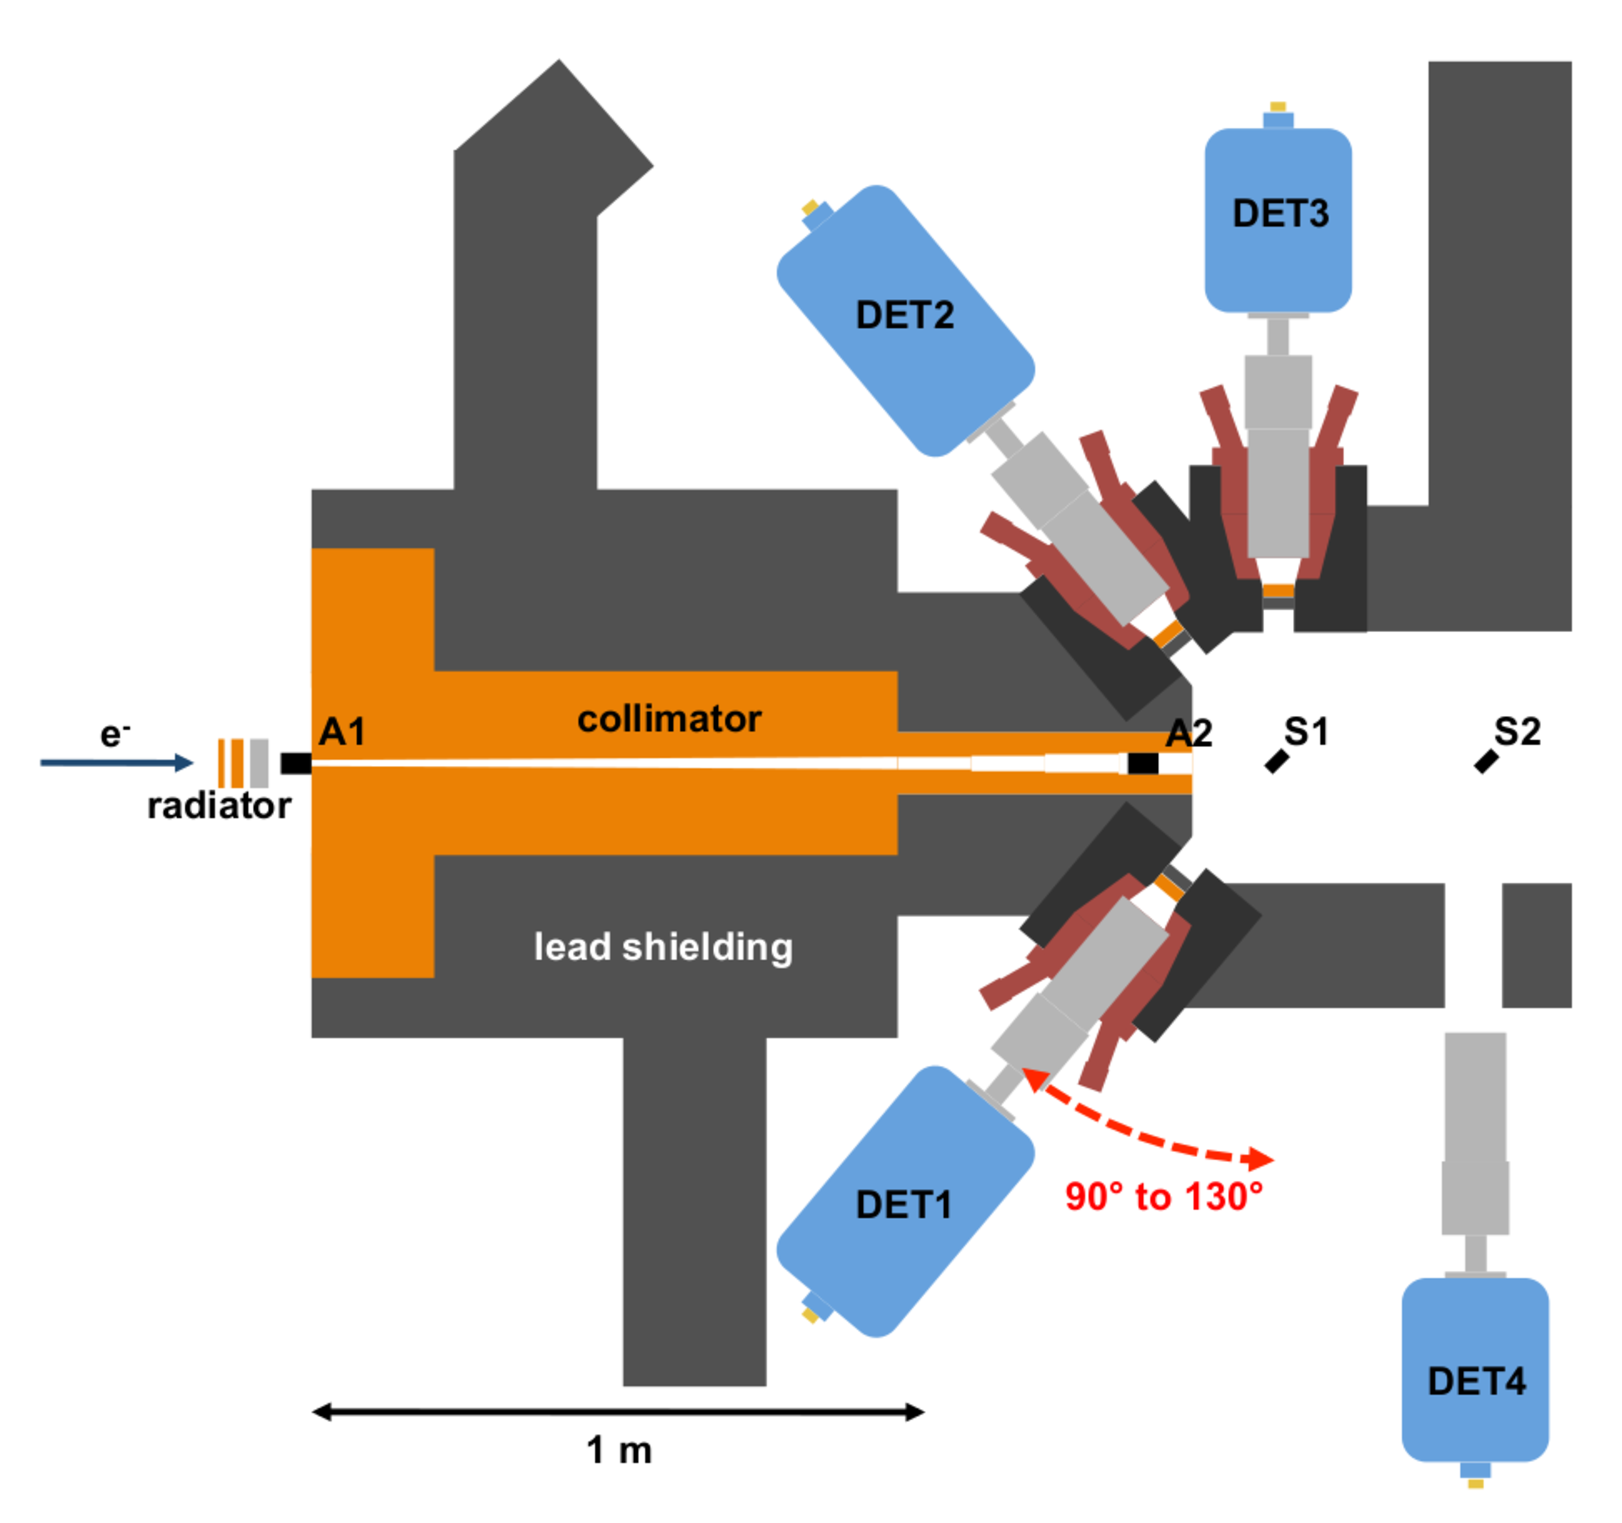
\includegraphics[width=\textwidth]{figures/dhips.pdf}
\end{textblock}

\begin{textblock}{6.}(9., -5.)
    \begin{itemize}
        \item Hayward et al. (1957)
        \item Continuous spectrum of photons up to the maximum electron energy
    \end{itemize}
\end{textblock}

\def \SPECTRUMX {9.}
\def \SPECTRUMY {0.}

\begin{textblock}{6.}(\SPECTRUMX, \SPECTRUMY)
    \visible<2>{
        \includegraphics[width=\textwidth]{figures/python/bremsstrahlung_linear.pdf}
    }
\end{textblock}

\begin{textblock}{6.}(\SPECTRUMX, \SPECTRUMY)
    \visible<3>{
        \includegraphics[width=\textwidth]{figures/python/bremsstrahlung_logarithmic.pdf}
    }
\end{textblock}